\documentclass[utf8]{ctexbook}
%\usepackage[utf8]{ctex}
\usepackage{euscript}
\usepackage{graphicx}
\usepackage{mathrsfs}
\usepackage{amssymb}
\usepackage{amsmath}
\numberwithin{equation}{section}
\usepackage{wrapfig}
\usepackage{hyperref}
\usepackage[all]{hypcap}
\hypersetup{hypertex=true,
            colorlinks=true,
            linkcolor=red,
            anchorcolor=blue,
            citecolor=red}
\usepackage{theorem}
\newtheorem{proposition}{命题}[chapter]
\title{旋量和时空\\卷1}
\author{Roger Penrose \\Wolfgang Rindler\\limbo137 译}
\begin{document}
\maketitle
\tableofcontents
\chapter*{前言}
  高度准确地说,我们所居住的时空可以看作是一个光滑的四维流形,并赋予了爱因斯坦狭义或广义相对论的光滑洛伦兹度规。当然,用于流形及其度规的数学处理最常用的形式是张量分析(或诸如Cartan的活动标架微积分之类的基本等效的替代品)。但是在四个维度和洛伦兹度量的特定情况下,碰巧存在(出于偶然或天意)另一种形式,这种形式在许多方面都更合适,那就是2-旋量的形式。然而,即使在Cartan首次提出一般旋量概念70年前,2-旋量分析仍相对陌生。自Dirac在其电子方程式中揭示自旋在相对论物理学中起着根本性的重要作用之后的70年左右,Van Der Waerden提供了基本的2-旋量代数和表示法。
  
  编写本书的目的是希望使这些想法更加流行。我们会假设读者没有知识的情况下相当详细地研究2-旋量分析,并说明如何将其视为对更熟悉的世界张量分析的有用补充或实用替代。在这里,我们将全神贯注于2-旋量,而不是4-旋量,这些4-旋量已经成为理论物理学家更为熟悉的工具。其原因是,只有2-旋量才能获得标准矢量张量分析的一种实用替代方案,其中2-旋量是最原始的元素,从中可以容易地获得4-旋量(以及张量)内置的。
  
  旋量分析可以被认为比标准的世界张量分析所描述的应用了更深的时空结构。相比之下,世界张量的精炼程度较低,无法使量子力学特别给光带来的时空的某些微妙特性透明化,而且尤其是使某些类型的数学计算异常繁重。(它们的优势在于可应用于任意尺寸的流形,而不是提供特定的时空演算。)
  实际上,通过明确的规定,任何张量计算都可以完全转换为2-旋量形式。从某种意义上说,反之亦然-我们将在本书的后面对这种翻译进行全面的处理-尽管简单的自旋操作的张量翻译可能会变得极其复杂。这种有效的对等可能导致一些“怀疑论者”相信棘手是“不必要的”。我们希望这本书能够帮助说服读者相信,如果只有张量方法可用,那么关于时空的许多旋转性结果将无法发现,而其他一些先因和相互关系将被张量描述完全掩盖。
  
  如果适当地考察一下,则2-旋量分析也比张量分析更简单。根本原因是基本自旋空间是二维复杂的,而不是真实的四维的。二维不仅比四维更容易处理,而且复杂的代数和复杂的几何图形具有许多简单,优雅和统一的特性,而这是它们的真实对手所没有的。
  
  此外,旋量似乎与量子力学中出现的复数有着深远的联系\footnote{关于时空几何以及量子理论可能由潜在的复杂性而不是实际结构支配的观点在扭量理论中得到了进一步发展,这只是本卷中讨论的几个主题之一。《旋量与时空》卷2:时空几何中的旋量和扭量方法,(剑桥大学出版社,1985年)}。尽管在这项工作中,我们不会像这样关注量子力学,但实际上,我们描述的许多技术在量子环境中都非常有价值。虽然我们的讨论将完全以经典方式进行,但形式上可以在没有本质困难的情况下适用于量子(或量子场理论)问题。
  
  据我们所知,这本书是第一本介绍使用2-旋量对时空几何进行全面研究的书。我们的演示文稿中还有其他几个新功能。其中之一是对张量和旋量分析系统地和一致地使用抽象指标方法。我们希望,随随便便翻阅本书的纯粹的微分几何学不会因众多指标的出现而自动退缩。除了偶尔用粗体显示的竖立指标外,我们的指标与更常见的指标不同,它们是抽象的标记,没有参考任何基准或坐标系。我们对抽象指标的使用导致了传统处理方法的许多简化。实际上,某种指标标记的使用似乎实际上是必不可少的,以便可以以透明的形式呈现必要的详细操作。(在附录中,我们概述了一种替代的等效图表符号,这对计算非常有用。)
  
  这本书在介绍其他几个主题时似乎也正在开辟一些新领域。我们不仅提供2-旋量本身的显式几何实现,而且还提供其各种代数运算以及一些相关拓扑的显式几何实现。我们为旋量和一般张量代数给出了一系列有用的引理。我们提供了对自旋系数(不一定是归一化的)的第一个综合处理,其中包括压缩的自旋加权和boost加权算子$\eth$和$\mathcal{P}$以及它们的保形不变修正$\eth_\mathscr{C}$和$\mathcal{P}_\mathscr{C}$。我们介绍保形不变性的一般处理;以及电磁场和Yang-Mills领域的抽象索引运算符方法(我们希望后者的外观有些笨拙,但可以通过我们的方案的全面性来弥补)。我们认为(自加权)球形谐波的旋量对待是新的。我们以前没有以书本形式出现过精确的场集合,这些场是唯一远离光锥上任意选择的空数据传播的系统。也没有相关的显式积分旋子公式(广义的Kirchhoff-d'Adhemar表达式)来表示无质量的自由场。我们首次提出了相互作用的麦克斯韦-狄拉克理论的发展,该理论是由之字形和叉形零路径描述的积分之和得出的。
  
  至于这项工作的起源,可以追溯到1962年春天,当时我们一个人(RP)举办了一系列有关当时相对论中的2旋量的研讨会,另一个人(WR)进行了笔记和越来越相信这些笔记可能会成为一本书。那个夏天的早期章节的重复草稿已分发给同事。随着主题的发展,我们在随后的草案中所做的努力在随后的几年中不断增加和减弱。最后,在过去的三年中,我们共同努力,重新编写,几乎使整个工作翻了一番,并希望将其完全更新。在其风格上,我们试图保留原始研讨会的某种非正式且宽松的方式,清楚地说明了我们的动机,没有回避对某些数学结果的启发式辩护,并且偶尔会切线或沉迷于旁白。存在许多更快速,更简洁的方式来达到要求的形式,但是我们更喜欢悠闲地步伐,一方面是为了促进学生自学的发展,另一方面是强调该主题的脚踏实地的实用性。
  
  幸运的是,我们相当冗长的手稿允许将自然分为两卷,现在可以独立阅读。第1卷的简介部分概述了图1。2.第1卷中的参考文献。1至第6-9章参考卷1。2。
  
  我们要感谢许多人。我们提到的那些人是最容易想到的具体贡献者,不可避免的是,在我们从事这项工作的二十多年中,有些名字已经逃脱了我们的记忆。对于各种不同的帮助,我们感谢Nikos Batakis,Klaus Bichteler,Raoul Bott,Nick Buchdahl,Subrahmanyan Chandrasekhar,Jurgen Ehlers,Leon Ehrenpreis,Robert Geroch,Stephen Hawking,Alan Held,Nigel Hitchin,Jim Isenberg,Ben Jeffryes,Saunders Mac Lane,Ted Newman,Don Page,Felix Pirani,Ivor Robinson,Ray Sachs,Engelbert Schiicking,William Shaw,Takeshi Shirafuji,Peter Szekeres,Paul Tod,Nick Woodhouse,尤其是Dennis Sciama一直以来的不懈鼓励。我们还要感谢Markus Fierz引致第321页脚注的评论。特别要热烈感谢Judith Daniels在写作经历艰难时期时对手稿的鼓励和详尽批评。我们也非常感谢邹上俊在参考和相关事务方面的贴心帮助。最后,对于那些我们无法再回想起来的人,我们表示感谢和歉意。
  
  1984
  \\Roger Penrose \\Wolfgang Rindler
\chapter{世界矢量和自旋矢量的几何}
\section{Minkowski矢量空间}\label{sec:11}

在本章中,我们关注与世界矢量空间有关的几何。该空间称为Minkowski矢量空间。它由相对论时空中的位置矢量集合组成,原点来自任意选择的起源事件。在广义相对论的弯曲时空中,Minkowski向量空间作为时空点(事件)的切空间出现。其他情形是四速度和四动量所张成的空间。

Minkowski矢量空间是实数域$\mathbb{R}$上的四维矢量空间$\mathbb{V}$,$\mathbb{V}$是具有定向,号差为$(+,-,-,-)$的(双线性)内积还有时间定向。(这些术语的确切含义下面都会讲到。)因此,对于任何向量空间,我们都有加法和标量乘法,对于所有的$\mathbf{U},\mathbf{V},\mathbf{W}\in\mathbb{V},a,b\in \mathbb{R}$满足
    \begin{gather}
        \mathbf{U}+\mathbf{V}=\mathbf{V}+\mathbf{U},\mathbf{U}+(\mathbf{V}+\mathbf{W})=(\mathbf{U}+\mathbf{V})+\mathbf{W}\notag \\
        a(\mathbf{U}+\mathbf{V})=a\mathbf{U}+a\mathbf{V},(a+b)\mathbf{U}=a\mathbf{U}+b\mathbf{U}\notag \\
         a(b\mathbf{U})=(ab)\mathbf{U},1\mathbf{U}=\mathbf{U},0\mathbf{U}=0\mathbf{V}=:\mathbf{0}
    \end{gather}
$\mathbf{0}$是加法的中性元素。通常,我们将$-\mathbf{U}$表示为$(-1)\mathbf{U}$,我们采用通常意义下的减法和括号的约定,例如$\mathbf{U}+\mathbf{V}—\mathbf{W}=(\mathbf{U}+\mathbf{V})+(-\mathbf{W})$等。

\(\mathbb{V}\)的四维性等效于存在由四个线性无关的向量$\mathbf{t},\mathbf{x},\mathbf{y},\mathbf{z}\in\mathbb{V}$.也就是说,任何$\mathbf{U}\in\mathbb{V}$都可以以以下形式唯一表示
\begin{equation}
    \mathbf{U}=U^0\mathbf{t}+U^1\mathbf{x}+U^2\mathbf{y}+U^3\mathbf{z} \label{eq:fenliang}
\end{equation}
坐标为$U^0,U^1,U^2,U^3\in\mathbb{R}$;只有0的所有坐标均为零。$\mathbb{V}$的任何其他基数也必须具有四个元素,并且$\mathbb{V}$中任何一个由四个线性无关元素构成的集合也是一组基。我们经常用$\mathbf{g_i}$表示$\mathbb{V}$的基$(\mathbf{t},\mathbf{x},\mathbf{y},\mathbf{z})$,其中
\begin{equation}
    \mathbf{t}=\mathbf{g_0},\mathbf{x}=\mathbf{g_2},\mathbf{y}=\mathbf{g_2},\mathbf{z}=\mathbf{g_3} \label{eq:113}
\end{equation}
然后(\ref{eq:fenliang})变成
\begin{equation}
    \mathbf{U}=U^0\mathbf{g_0}+U^1\mathbf{g_1}+U^2\mathbf{g_2}+U^3\mathbf{g_3}\label{eq:114}
\end{equation}
这里我们使用爱因斯坦求和约定,从今往后:当指标在一项中出现两次,一次在上,一次在下时,它意味着对这个指标求和。粗体字竖立的小写拉丁字母指标$\mathbf{a},\mathbf{i},\mathbf{a_0},\mathbf{a_1},\mathbf{\hat{a}}$等,将始终被理解为包含四个值0,1,2,3.稍后,我们还将使用粗体字竖立的大写拉丁字母$\mathbf{A},\mathbf{I},\mathbf{A_0},\mathbf{A_1},\mathbf{\hat{A}}$等,用于仅在两个值$0,1$范围内的指标。同样,求和约定仍将适用。

考虑$\mathbb{V}$的两组基,比如$(\mathbf{g_0},\mathbf{g_1},\mathbf{g_2},\mathbf{g_3})$和$(\mathbf{g_{\hat{0}}},\mathbf{g_{\hat{1}}},\mathbf{g_{\hat{2}}},\mathbf{g_{\hat{3}}})$。请注意,我们使用“标记指标”表示法,其中指标(而不是不同基的核心字母等)带有区别标记(帽子等)。像$\mathbf{a},\mathbf{\hat{a}},\mathbf{\hat{\hat{\hat{a}}}}$等的指标在数值上与$\mathbf{a},\mathbf{b},\mathbf{c}$无关。读者一开始可能会觉得这种表达方式不美观,但是习惯它是值得的。其优势后面就会显现。现在,第一个基的每个向量$\mathbf{g_i}$可以表示成第二个基的向量$\mathbf{g_{\hat{i}}}$的线性组合
\begin{align}
    \mathbf{g_i}&=g_{i}^{\hat{0}}\mathbf{g_{\hat{0}}}+{g_{i}^{\hat{1}}}\mathbf{g_{\hat{1}}}+{g_{i}^{\hat{2}}}\mathbf{g_{\hat{2}}}+{g_{i}^{\hat{3}}}\mathbf{g_{\hat{3}}}\notag \\
    &={g_{i}^{\hat{j}}}\mathbf{g_{\hat{j}}}
\end{align}
${g_{i}{}^{\hat{j}}}\mathbf{g_{\hat{j}}}$的16个分量形成一个($4 \times 4$)实非奇异矩阵。因此det(${g_{i}{}^{\hat{j}}{}}$)非零。如果为正,则称\(\mathbf{g_i}\)和\(\mathbf{g_{\hat{i}}}\)具有相同的定向;若为负,则称这两组基具有相反的定向。注意,“具有相同定向”的关系是等价关系。因为若$\mathbf{g_{\hat{i}}}=g_{\hat{i}}{}^{j}\mathbf{g_{j}}$,则$g_{\hat{i}}{}^j$和$g_{i}{}^{\hat{j}}$是逆矩阵,因此它们的行列式具有相同的符号;若\(\mathbf{g}_i=g_{i}{}^{\hat{\hat{j}}}\mathbf{g}_{\hat{\hat{j}}}\)且\(\mathbf{g}_{\hat{i}}=g_{\hat{i}}{}^{\hat{\hat{j}}}\mathbf{g}_{\hat{\hat{j}}}\),则矩阵$(g_{i}{}^{\hat{\hat{j}}})$是$(g_{i}{}^{\hat{j}})$和$(g_{\hat{i}}{}^{\hat{\hat{j}}})$的乘积,因此如果两者都具有正的行列式,那么乘积的行列式也为正。因此,所有的基可分为两个不相交的等价类。我们称一类恰当的基,另一类为非恰当的基。正是这种选择为$\mathbb{V}$赋予了定向。

$\mathbb{V}$上的一个内积算子是指给$\mathbb{V}$中任意一对$\mathbf{U},\mathbf{V}$分配一个实数,记作$\mathbf{U} \cdot \mathbf{V}$,使得
\begin{equation}
    \mathbf{U}\cdot \mathbf{V}=\mathbf{V}\cdot \mathbf{U},(a\mathbf{U})\cdot \mathbf{V}=a(\mathbf{U}\cdot \mathbf{V}),(\mathbf{U}+\mathbf{V})\cdot \mathbf{W}=\mathbf{U}\cdot \mathbf{W}+ \mathbf{V}\cdot \mathbf{W}
\end{equation}
这个运算是对称且双线性的。我们还要求内积具有号差$(+---)$。这意味着存在一个基$(t,x,y,z)$使得
\begin{align}
    t\cdot t&=1,x\cdot x=y\cdot y=z\cdot z =-1\label{eq:117}\\
    t\cdot x&=t\cdot y =t\cdot y=t\cdot z = x\cdot y = x\cdot y =x\cdot z =y\cdot z=0\label{eq:118}
\end{align}
如果根据(\ref{eq:113})那样的形式表示该基,则可以简洁地将(\ref{eq:117})和(\ref{eq:118})改写为
\begin{equation}
    \mathbf{g}_i \cdot \mathbf{g}_j=\eta_{ij} \label{eq:119}
\end{equation}
矩阵$(\eta_{ij})$由下式给出
\begin{equation}
    (\eta_{ij})=(\eta^{ij})=\begin{pmatrix}
        1&&&\\
        &-1&&\\
        &&-1&\\
        &&&-1\\
    \end{pmatrix}
    \label{eq:1110}
\end{equation}

(为了符号一致性,稍后将需要使用升指标的版本 $\eta^{ij}$ )我们称满足(\ref{eq:119})的基称为Minkowski基。对于给定的实向量空间,众所周知\footnote{Sylvester的“号差惯性”定理},对于所有正交基(即满足(\ref{eq:118})的那些),正的自内积(\ref{eq:117})是不变的。

给定任何Minkowski基$\mathbf{g}_i$,根据(\ref{eq:114}),我们可以通过其对应的Minkowski坐标表示任何向量$\mathbf{U} \in \mathbb{V}$,然后内积为
\begin{align}
    \mathbf{U}\cdot \mathbf{V}&=(U^i\mathbf{g}_i)(V^j\mathbf{g}_j)=U^iV^j(\mathbf{g}_i\mathbf{g}_j)\\
    &=U^iV^j \eta_{ij}\\
    &=U^0V^0-U^1V^1-U^2V^2-U^3V^3 \label{eq:1111}
\end{align}
注意到$\mathbf{U}\cdot \mathbf{g}_j=U^i\eta_{ij}$,于是
\begin{equation}
    U^0 = \mathbf{U}\cdot \mathbf{g}_0,U^1 = -\mathbf{U}\cdot \mathbf{g}_1,U^2 = -\mathbf{U}\cdot \mathbf{g}_2,U^3 = -\mathbf{U}\cdot \mathbf{g}_3
\end{equation}
一个特殊情形是洛伦兹范数
\begin{equation}
    \lVert U\rVert =\mathbf{U}\cdot \mathbf{U} =U^iU^j\eta_{ij}=(U^0)^2-(U^1)^2-(U^2)^2-(U^3)^2\label{eq:1113}
\end{equation}
我们甚至可以根据洛伦兹范数来定义内积,即
\begin{equation}
    \mathbf{U}\cdot \mathbf{V}=\frac12 \{\lVert U+V\rVert-\lVert U\rVert-\lVert V\rVert \}\label{eq:1114}
\end{equation}
向量$\mathbf{U}\in \mathbb{V}$称为
\begin{equation}
    \begin{cases}
     \text{类时的}&\text{当}\left\lVert \mathbf{U}\right\rVert < 0\text{时} \\
     \text{类空的}&\text{当}\left\lVert \mathbf{U}\right\rVert > 0\text{时}\\
     \text{类光的}&\text{当}\left\lVert \mathbf{U}\right\rVert = 0\text{时}\\
    \end{cases} 
\end{equation}
就其Minkowski坐标而言,如果满足以下条件,则$\mathbf{U}$是有因果性的(类时或类光)
\begin{equation}
    (U^0)^2\geqslant (U^1)^2+(U^2)^2+(U^3)^2\label{eq:116}
\end{equation}
等号在U为类光时取得,如果U和V均为因果的,则结合(\ref{eq:116})和Schwarz不等式,我们得到
\begin{align}
    \lvert U^0V^0 \rvert&\geqslant\{(U^1)^2+(U^2)^2+(U^3)^2\}^{\frac{1}{2}}\{(V^1)^2+(V^2)^2+(V^3)^2\}^{\frac{1}{2}}\\
    &\geqslant U^1V^1+U^2V^2+U^3V^3
\end{align}
因此,除非U和V都为零并且彼此成正比,或者除非其中一个为零(这两个不等式都取得等号),否则根据(\ref{eq:1111}),$\mathbf{U}\cdot \mathbf{V}$的符号为与$U^0V^0$的符号相同。因此,除非两个非零因果矢量为类光的且成比例,否则它们不能正交。

我们可以把因果性向量分成两个不同的类中,同类的两个向量的内积为正数,而不同类的两个向量的内积为负。这两个类是根据$U_0$的符号来区分的,$U_0$为正的类就是类时基向量$\mathbf{t=g_0}$所在的类。$\mathbb{V}$的时间定向指称第一个类中的元素为未来指向的,另一个类的元素称为过去指向的。我们经常把指向未来的时间型[类光,因果]向量简单地称为未来类时型[-类光,-因果]向量。如果$\mathbf{t}$是一个未来类时的矢量,那么Minkowski基(t, x, y, z)就称为\textbf{正时的}。当提到一个正时的Minkowski基时,未来因果性向量就是$U_0 > 0$的那些。零向量虽然是类光的,但既不是未来类光的也不是过去类光的。任何未来因果向量的和$-1$的乘积都是过去因果向量。

$\mathbb{V}$的空间定向指每个闵可夫斯基的三个空间向量分配“右手性”或“左手性”。这可以通过$\mathbb{V}$的定向向和时间定向来实现。
因此,如果Minkowski基$\mathbf{(t,x,y,z)}$既是恰当的又是正时的,或是非恰当的又是非正时的,则空间基$\mathbf{(x, y, z)}$被称为右手性。否则空间基$\mathbf{(x, y, z)}$是左手的,Minkowski基既是恰当的又是正时的,称作受限的。$\mathbb{V}$的任何两个方向,时间方向和空间方向决定了第三个方向,如果任意两个方向相反,第三个必须保持不变。为了在我们所在的时空做出这些选择,我们最好是首先选择一个空间基$\mathbf{(x, y, z)}$然后根据知名物理学家使用标准和大多数人的写字习惯用手的结构称它为左手或是右手性的\footnote{针对弱相互作用(P)在空间反射下和$K^0$-衰变在空间反射和正反粒子交换(CP)下非不变(不守恒)的性质,或许现在可以确认物理时空的这种的空间定向独立于文化或生理因素:参见
Lee and Yang (1956), Wu, Ambler, Hayward Hoppes and Hudson (1957), Lee, Oehme and Yang (1957), christensen, Cronin, Fitch and Turlay (1964), Wu and Yang (1964):
也有Gardner(1967),作为一个受欢迎的说法}。类似地,统计物理学也决定了一种独特的未来感。

如前所述,闵可夫斯基向量空间$\mathbb{V}$可以看作是构成闵可夫斯基时空$\mathbb{M}$的点(事件)相对于任意原点的位置向量空间。这个时空是狭义相对论的舞台。没有任何一个点是特殊的,原点也不是:它在平移下是不变的,也就是说,它是一个仿射空间。
即$\mathbb{M}$和$\mathbb{V}$之间的关系可以通过这样一个映射被描述出来
\begin{equation}
    \mathrm{vec}:\mathbb{M}\times \mathbb{M}=\mathbb{V}
\end{equation}
满足
\begin{equation}
    \mathrm{vec}(P,Q) +\mathrm{vec}(Q,R) = \mathrm{vec}(P,R)\label{eq:1119}
\end{equation}
其中$\mathrm{vec} (P,P)=0, \mathrm{vec}(P,Q)=-\mathrm{vec}(Q, P)$,我们可以把$\mathrm{vec}(P, Q)$看作Q相对于P的位置向量$\overrightarrow{PQ}\in \mathbb{V} $,其中$P, Q\in \mathbb{M}$。
显然,$\mathbb{V}$通过这个映射得出一个范数,这里称为线长,对任意点$P,Q \in \mathbb{M}$:
\begin{equation}
    \Phi (P,Q):= \left\lVert \mathrm{vec} (P,Q)\right\rVert \label{eq:1120}
\end{equation}
对于$\mathbb{M},\mathbb{M}\leftrightarrow \mathbb{R}^4$的标准坐标化,其中$\mathbb{R}^4$是实数的四维空间,由原点$O$的选择和Minkowski基$\mathbf{g_i}=\overrightarrow{OQ}_i,Q_0,Q_1,Q_2,Q_3\in \mathbb{M}$的选择组成。任意点$P\in\mathbb{M}$的坐标$P^0, P^1 ,P^2 ,P^3$就是
向量$\overrightarrow{OP}$在$\mathbf{g_i}$下的坐标,即$\overrightarrow{OP} = P^\mathbf{i}\mathbf{g_i}$。在(\ref{eq:1119})中我们发现,用$O$代替$Q$,得到$\overrightarrow{PR}$相对于$\mathbf{g_i}$的坐标如下:
\begin{equation}
    (\overrightarrow{PR})^i = R^i-P^i\label{eq:1121}
\end{equation}
显然与原点的选择无关。将此和(\ref{eq:1120})代入(\ref{eq:1113})得到
\begin{equation}
    \Phi (P,Q):=(Q_0-P_0)^2 - (Q_1-P_1)^2  - (Q_2-P_2)^2 - (Q_3-P_3)^2 
\end{equation} 
V的线性自变换保持了洛伦兹范数不变,因此,通过(\ref{eq:1114}),也就是内积,称为(活动)洛伦兹变换。如果这样的变换保持了$\mathbb{V}$的定向和时间定向,则称为受限洛伦兹变换。显然,[受限的]洛伦兹变换形成一个群,这个群称为[受限的]洛伦兹群。类似地,$\mathbb{M}$的保持线长不变的自变换(这里不需要线性假设)称为(主动)Poincaré变换。任何这样的变换都会在V上产生一个洛伦兹变换,因此也可以再一次划分为受限或非受限。受限制的Poincaré变换显然形成了一个群\footnote{注意我们使用只能在Minkowski矢量空间上的六参数齐次群使用“洛伦兹变换”这个名词,而Minkovski时空上的十参数非齐次群则称为Poincaré变换}

在我们惯常的Minkovski时空中进行的任何物理实验都可能“被”Poincaré变换,即在空间中旋转,在空间和时间中平移,并给出一个一致的运动结果。这是狭义相对论的基础,它不依赖参考系或其他物理定律。

\subsection*{坐标变换}
如果没有进一步的规定,洛伦兹和Poincaré变换在本书中都将被理解为是主动的。但有时考虑“被动的”洛伦兹(和Poincaré)变换是有用的。这些是坐标空间$\mathbb{R}^4$的变换。$\mathbb{V}$(或$\mathbb{M}$)的重坐标化,任意$\mathbb{V}$中的Minkowski基$\mathbf{g_i}$(或$\mathbb{M}$中的基$\mathbf{g_i}$和原点$O$)为每个$\mathbb{V}$上的 $\mathbf{U}$ (或$\mathbb{M}$上的 $\mathbf{U}=\overrightarrow{OP}$)定义了一组坐标$U^i$的四维基,$\mathbf{U}=U^\mathbf{i}\mathbf{g_i}$。参考系的变化,也就是$\mathbb{V}$中的$\mathbf{g_i}\mapsto \mathbf{g_{\hat{i}}}$(或$\mathbb{M}$中的基$\mathbf{g_i}$和原点$O$)导致了$\mathbb{V}( \text{或} \mathbb{M})$的坐标变化。由此产生的关联
\begin{align}
    G:&U^i\mapsto U^{\hat{i}}\label{eq:1123}\\
    (\text{或}U^i\mapsto U^i&+K^i, K^i \text{是常数}) \nonumber
\end{align}
被称为被动洛伦兹(或Poincaré)变换。如果它可以由两个受限的闵可夫斯基基$\mathbf{g_i}$和$\mathbf{g_{\hat{i}}}$生成,则称其为受限的。为了简洁起见,我们现在将集中讨论洛伦兹变换,推广到Poincaré变换是容易的。

这两个参考系是由
\begin{equation}
    \mathbf{g_i}={g_{i}{}^{\hat{i}}}\mathbf{g_{\hat{i}}}\label{eq:1124}
\end{equation}
关联起来的,那么
\begin{equation}
    \mathbf{U}=U^{\hat{i}}\mathbf{g_{\hat{i}}}=U^{i}\mathbf{g_i}=U^i g_{i}{}^{\hat{i}}\mathbf{g_{\hat{i}}}
\end{equation}
因此被动变换(\ref{eq:1123})由
\begin{equation}
    U^{\hat{i}}=U^i g_{i}{}^{\hat{i}}\label{eq:1125}
\end{equation}
明确给出,显然是线性的。由矩阵$g_{i}{}^{\hat{i}}$充分表征。
通过坐标的描述主动洛伦兹变换的做法,往往比较方便,但也有一点点误导(说误导是因为主动洛伦兹变换独立于所有坐标存在,而被动洛伦兹变换则不然。)
因此,对于给定的主动洛伦兹变换$L:\mathbf{U}\mapsto \mathbf{V}$,我们可以将$\mathbf{U}$及其像$\mathbf{V}$同时指向一个(任
\begin{figure}
    \centering
    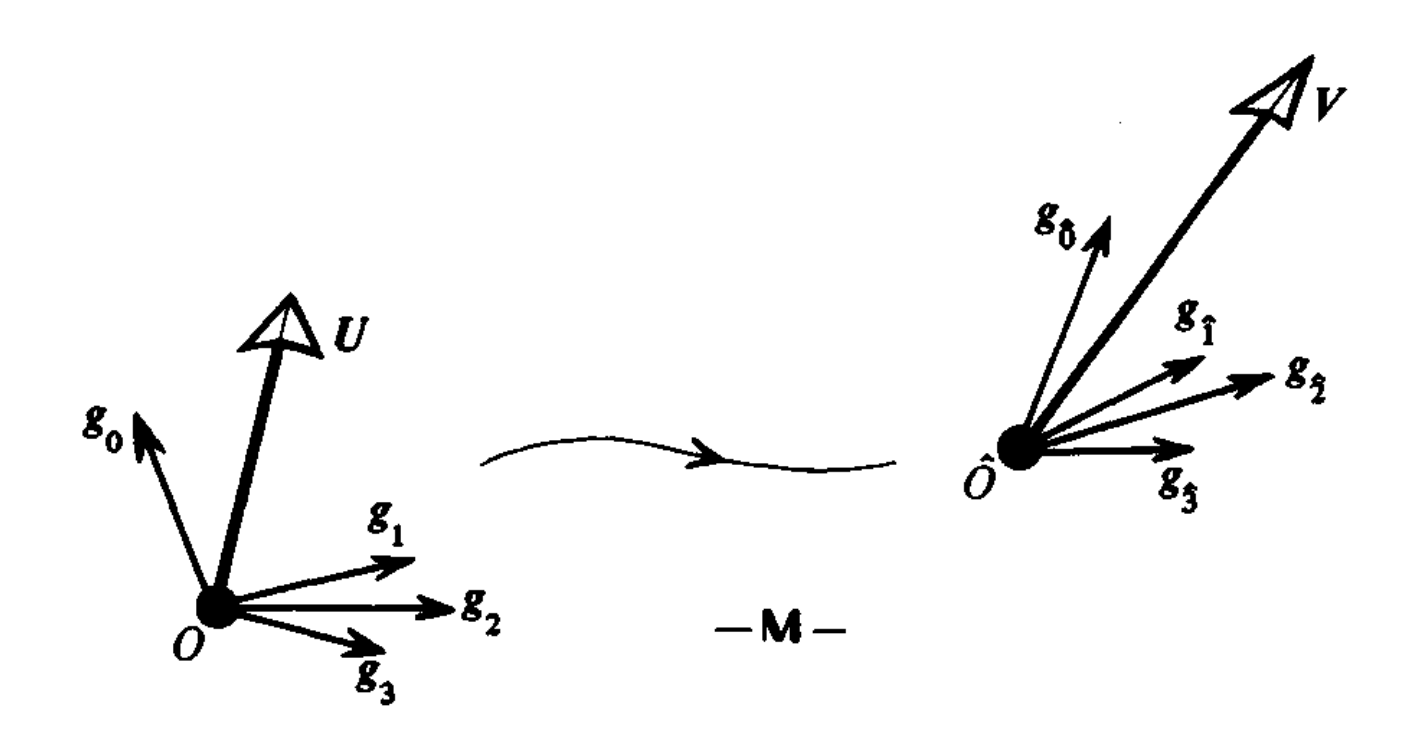
\includegraphics[width=10cm]{fg1-1.png}
    \caption{主动的Poincaré变换将$O$点的世界矢量$\mathbf{U}$变换到$\hat{O}$点的世界矢量$\mathbf{V}$。也把$O$点的基$\mathbf{g_i}$变换到$\hat{O}$点的基$\mathbf{g_{\hat{i}}}$,$\mathbf{g_i}$中$\mathbf{U}$的坐标$U^i$和$\mathbf{g_{\hat{i}}}$中$\mathbf{V}$的坐标$V^{\hat{i}}$是一样的;(即$U^i=V^{\hat{i}}$)。因此,由$\{\mathbf{g_i},O\}\mapsto \{\mathbf{g_{\hat{i}}},\hat{O}\}$诱导的(反向)被动变换把$\mathbf{U}$的坐标$U^i(=V^{\hat{i}})$变换到$\mathbf{V}$的原始坐标$V^i$}\label{fig:1-1}
\end{figure}
意的)Minkowski基$\mathbf{g_i}$,其在L下的原像为$\mathbf{g_i}$,如(\ref{eq:1124})。由于假设L的线性关系,$\mathbf{V}$在$\mathbf{g_{\hat{i}}}$下的表达式的分量必须与$\mathbf{U}$在$\mathbf{g_i}$下的表达式的分量相同,因此我们有,(参见(\ref{eq:1125}),也见图\ref{fig:1-1})
\begin{equation}
    U^{\hat{i}}=U^{j}g_{j}{}^{\hat{i}}=V^{\hat{j}}g_{j}{}^{\hat{i}}\label{eq:1126}
\end{equation}

这里违反了一般规则,但我们也理解了对不同的索引对$j$和$\hat{j}$的求和。因此,我们有如下的显式形式的变换\footnote{译者注:原文中(\ref{eq:1126})和(\ref{eq:1127})都没有中间项,是译者加的},
\begin{equation}
    V^{\hat{j}}=U^j=U^{\hat{i}}L_{\hat{i}}{}^{j}\label{eq:1127}
\end{equation}
其中
\begin{equation}
    (L_{\hat{i}}{}^{j})=(g_{j}{}^{\hat{i}})^{-1}\label{eq:1128}
\end{equation}
因此,将$\mathbf{g_i}$为$\mathbf{g_{\hat{i}}}$的主动洛伦兹变换$L$,在其对矢量坐标的影响上等价于从$\mathbf{g_{\hat{i}}}$到$\mathbf{g_i}$的变换诱导出的被动洛伦兹变换$G^{-1}$

如果L是一个受限的洛伦兹变换,它显然将一个受限的闵可夫斯基基变换到另一个受限的闵可夫斯基基,因此相应的被动变换$G$也是受限的。反过来,如果$G$是受限的,假设它是由受限的基$\mathbf{g_i}$和$\mathbf{g_{\hat{i}}}$产生的;那么对应的$L$保持范数,内积和定向,因为事实上它的坐标没有变,因此$L$是受限的。现在为了让$L$保持内积我们要求-由(\ref{eq:1111})和(\ref{eq:1127})摘掉帽子
\begin{equation}
    \eta_{ij}L_{k}{}^{i}L_{l}{}^{j}=\eta_{kl}
\end{equation}
把它看作矩阵方程,我们看到$\mathrm{det}(L)=\pm 1$。L是受限的的条件是
\begin{equation}
    \mathrm{det}(L_i{}^j)= 1, L_0{}^0 > 0
\end{equation}
由于(\ref{eq:1128}),同样的条件适用于被动受限洛伦兹变换的矩阵。当然,它们也可以直接从定义中派生出来:
\begin{equation}
    \eta_{ij}g_{\hat{i}}{}^{i}g_{\hat{j}}{}^{j}=\eta_{{\hat{i}{\hat{j}}}},\mathrm{det}(g_{\hat{i}}{}^{i})=1,g_{\hat{0}}{}^{0}>0\label{eq:1121}
\end{equation}
\section{类光方向和自旋变换}\label{sec:1.2}
在$\S$\ref{sec:11}中考虑了世界向量$\mathbf{U}$在闵可夫斯基坐标下的传统表示。现在我们来看看另一种用坐标表示世界向量的方法。特别地,我们将得到光锥(即全体类光向量的集合)用复数表示的坐标。这就引出了自旋矢量的概念。

为了避免不必要的指标,我们用$T,X,Y,Z$来代替在受限的Minkowski基$\mathbf{(t, x, y, z)}$下矢量$\mathbf{U}$的坐标$U^0,U^1,U^2,U^3$:
\begin{equation}
    \mathbf{U}= T\mathbf{t} +X\mathbf{x}+ Y\mathbf{y}+ Z\mathbf{z}\label{eq:121}
\end{equation}
对于类光向量,其坐标满足。
\begin{equation}
    T^2-X^2-Y^2-Z^2=0\label{eq:122}
\end{equation}

通常我们只考虑在(闵可夫斯基)时空原点处的类光方向,注意,$\pm \mathbf{U}$具有不同的(即相反的)方向。未来[过去]
\footnote{译者注:作者常用大片的方括号来表达“或”的逻辑关系,并且这种关系是局部关联的}
的类光方向我们看成某个抽象空间的元素,我们称之为$\mathscr{S}^+[\mathscr{S}^-]$。这两个空间可以在任何给定的坐标系$(T, X, Y, Z)$中用未来[过去]光锥(\ref{eq:122})的$S^+[S^-]$超平面$T=1[T=-1]$来表示。在欧几里得$(X, Y, Z)$空间$T=1 [T=-1]$中,$S+ [S-]$是一个球面的方程
\footnote{我们在这里保留小写字母$x, y, z$表示$S^+$和$S^-$上的坐标}
\begin{equation}
    x^2 + y^2 + z^2 = 1\label{eq:123}
\end{equation}
(见图\ref{fig:1-2})当然,任意经过$O$点的向量(\ref{eq:121})的方向(无论其是否类光),除非它位于超平面$T= 0$,否则可以用$T= 1$或$T=-1$的一点表示。U从原点出发的方向在适当的超平面上由点$(X/\left\lvert T\right\rvert , Y/\left\lvert T\right\rvert , Z/\left\lvert T\right\rvert )$表示。$S^-$的内部表示过去的类时方向集合,$S^2$的内部表示未来的类时方向集合。这些球体的外部表示类空方向
\begin{figure}
    \centering
    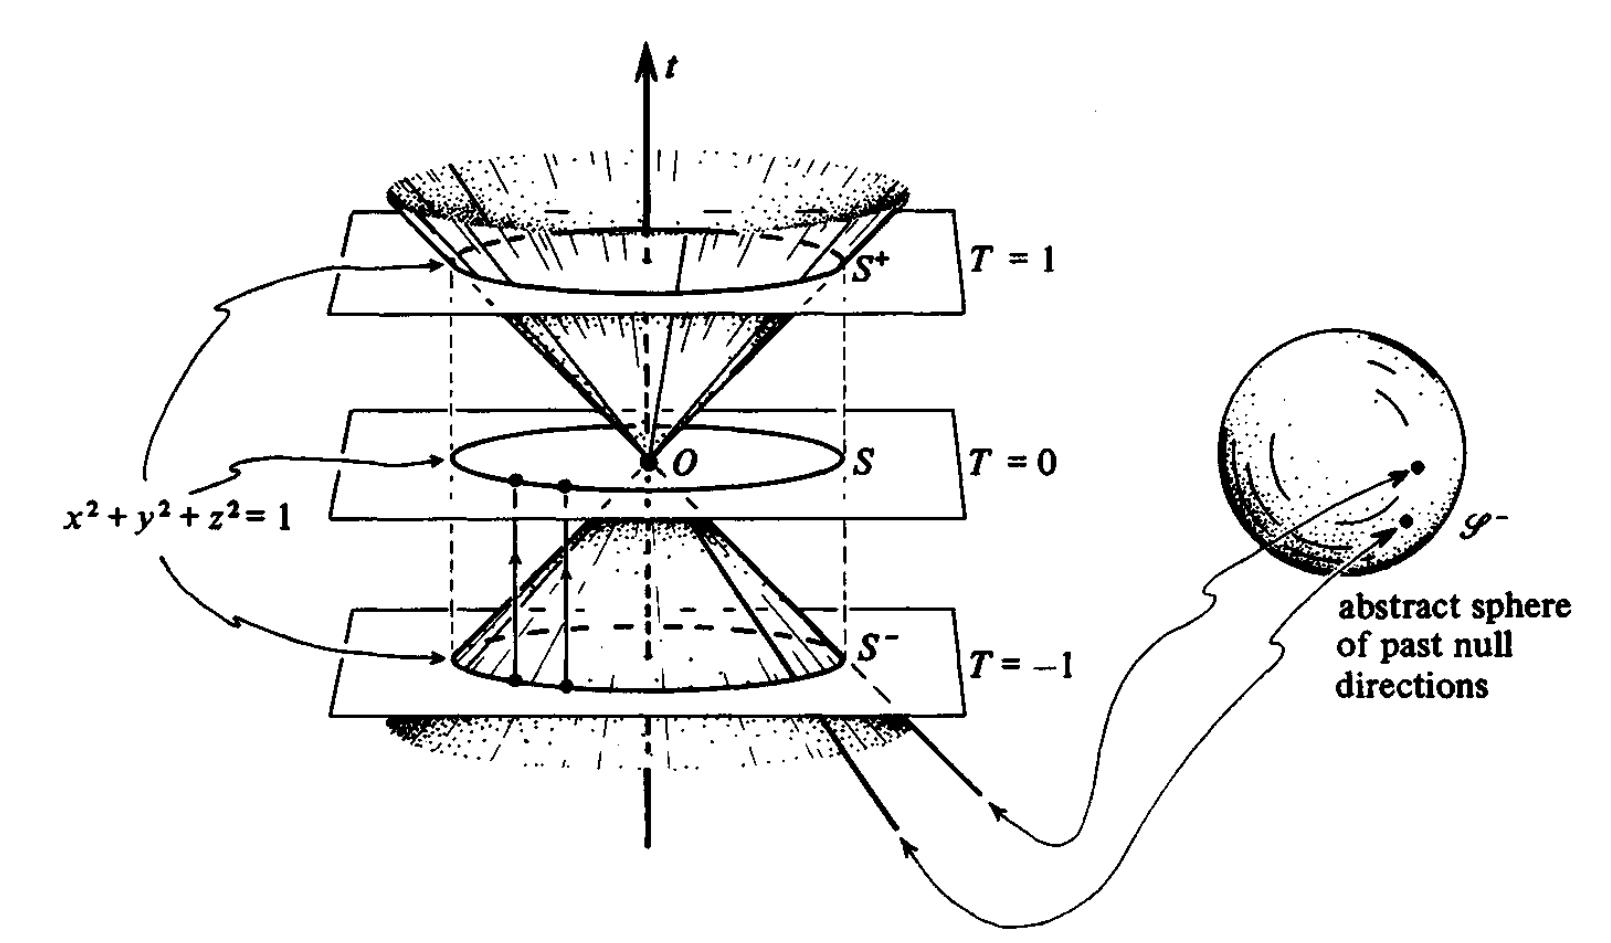
\includegraphics[width=12cm]{fig1-2.png}
    \caption{抽象的球体$\mathscr{S}^-$自然地表示了观察者的天球,而$S^-$,或者它对S的投影,给出了一个更具体的(尽管不那么守恒)的实现}\label{fig:1-2}
\end{figure}

让我们从物理的角度来考虑$S^-$和$S^+$的重要性。我们想象一个观察者位于时空中的事件$O$处。现在,通过他的眼睛的光线相当于通过$O$的类光直线,其过去的方向构成了观察者的视野。这是$\mathscr{S}^-$用球面$S^-$表示。事实上,$S^-$是相对于坐标架$(\mathbf{t,x,y,z})$静止的观察者真正“看到”的东西的一个精确的几何表示,也就是说,他的世界速度是$\mathbf{t}$。因为他可以想象自己永久位于中心的单位球(他的视野范围),他可以在任何瞬间把他所看到的画成一副图。从他的眼睛到$S$上这些像点的线是入射光线到他的瞬时空间$T=0$的世界线的投影。因此,这些像与$S^-$上的图像是一致的(参见图\ref{fig:1-2}),我们可以将$\mathscr{S}^-$或$S^-$称为O的\textbf{天球}。将$O$处过去的类光方向映射到$S^-$上的点,我们称之为\textbf{天空映射}。因为任何过去指向的类光向量$L$是唯一(且不变的)与一个指向未来的类光向量关联的,即$-L$,我们也用球面$S^+$来表示观察者的视野。我们可以称之为反天空映射。$S^+$和$S^-$之间的对应关系很简单,就是$(x,y,z)\leftrightarrow (-x,-y,-z)$,也就是说,如果我们把这两个球体叠加,就是对跖映射。这涉及到球的定向的逆转:例如,在$S^-$上的切向量从中心看顺时针旋转时,在$S^-$上逆时针旋转.

球面$S^+$(或$S^-$)可以很自然地看作是Argand(-Wessel-Gauss)平面\footnote{译者注:即复平面,下文中的复平面均指Argand平面}的黎曼球面,这个球面是包括无穷在内的复数的著名表示。我们熟悉的复平面及其黎曼球的性质反映了闵可夫斯基向量空间$\mathbb{V}$的诸多几何性质。特别是,$\mathbb{V}$上的受限洛伦兹变换被认为是由它对黎曼球面(以及上面的类光方向)的变动所唯一决定的。
此外,我们将在\S \ref{sec:1.4}中看到,自旋矢量可以在黎曼球面上得到一个相当直接的几何解释。

我们可以用一个复数替换$S^+$上的$x, y, z$坐标,这个复数是通过球面和平面之间的“立体对应关系”获得的(见图\ref{fig:1-3})。在$T=1$时的三维欧氏空间中画出平面$\Sigma$与方程$z = 0$ ,通过北极\footnote{我们选择北极而不是南极和大部分旋量的文献保持一致,也是因为它导致了在正向的相位变换下flag plane的右手性旋转(参见\S\ref{sec:1.4}\S\ref{sec:3.2})然而需要注意的是,当从外部看时,$S^+$的定向与从上方看$\Sigma$的定向相反。根据\S\ref{sec4.14}\S\ref{sec4.15}的约定,$\zeta$作为$S^-$上的反全纯坐标($S^-$上的全纯坐标)出现(参见图\ref{fig4-2}和图\ref{4-6})。}$N(1,0,0,1)$的投影把$S^+$映射到这个平面。让$P (1, x, y,z)$和$P'(1,X',Y',O)$表示$S^+$和$\Sigma$上的对应点,让点$A$和$B$分别表示从$P$到$CP'$,$CN$垂线的垂足。
用单个复参数
\begin{equation}
    \zeta=X'+\mathrm{i}Y'\label{eq:124}
\end{equation}
标记$\Sigma$上的点,我们有
\begin{figure}
    \centering
    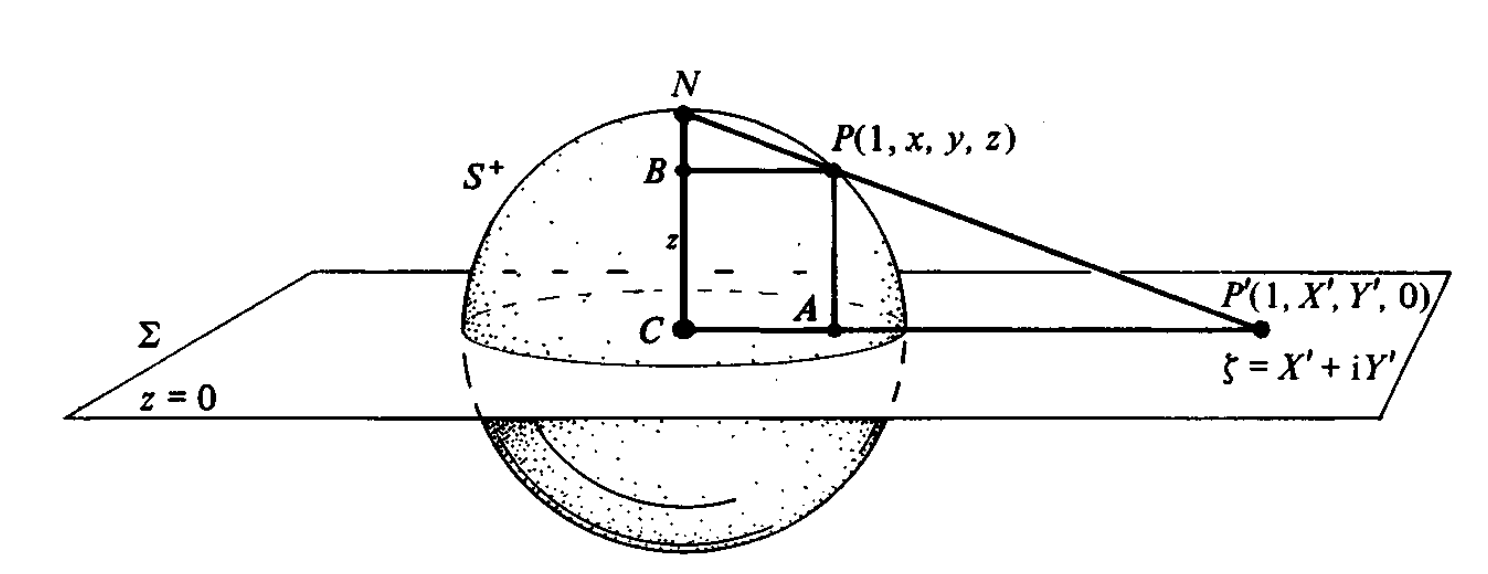
\includegraphics[width=12cm]{fig1-3.png}
    \caption{$S^+$到复平面的球极映射}\label{fig:1-3}
\end{figure}
\begin{equation}
    x+\mathrm{i}y=h\zeta\label{eq:125}
\end{equation}
其中
\[h=\frac{CA}{CP'}=\frac{NP}{NP'}=\frac{NB}{NC}=1-z\]
因此$P$点在坐标$(1,x,y,z)$下对应的$\zeta$的表达式就是
\begin{equation}
    \zeta =\frac{x+\mathrm{i}y}{1-z}\label{eq:126}
\end{equation}
为了获得逆关系,我们先利用(\ref{eq:123})在(\ref{eq:126})中消去x和y
\begin{equation}
    \zeta\bar{\zeta}=\frac{x^2+y^2}{(1-z)^2} =\frac{1+z}{1-z}\label{eq:127}
\end{equation}
在(\ref{eq:127})中反解出$z$,再代入(\ref{eq:126}) 我们得到
\begin{figure}
    \centering
    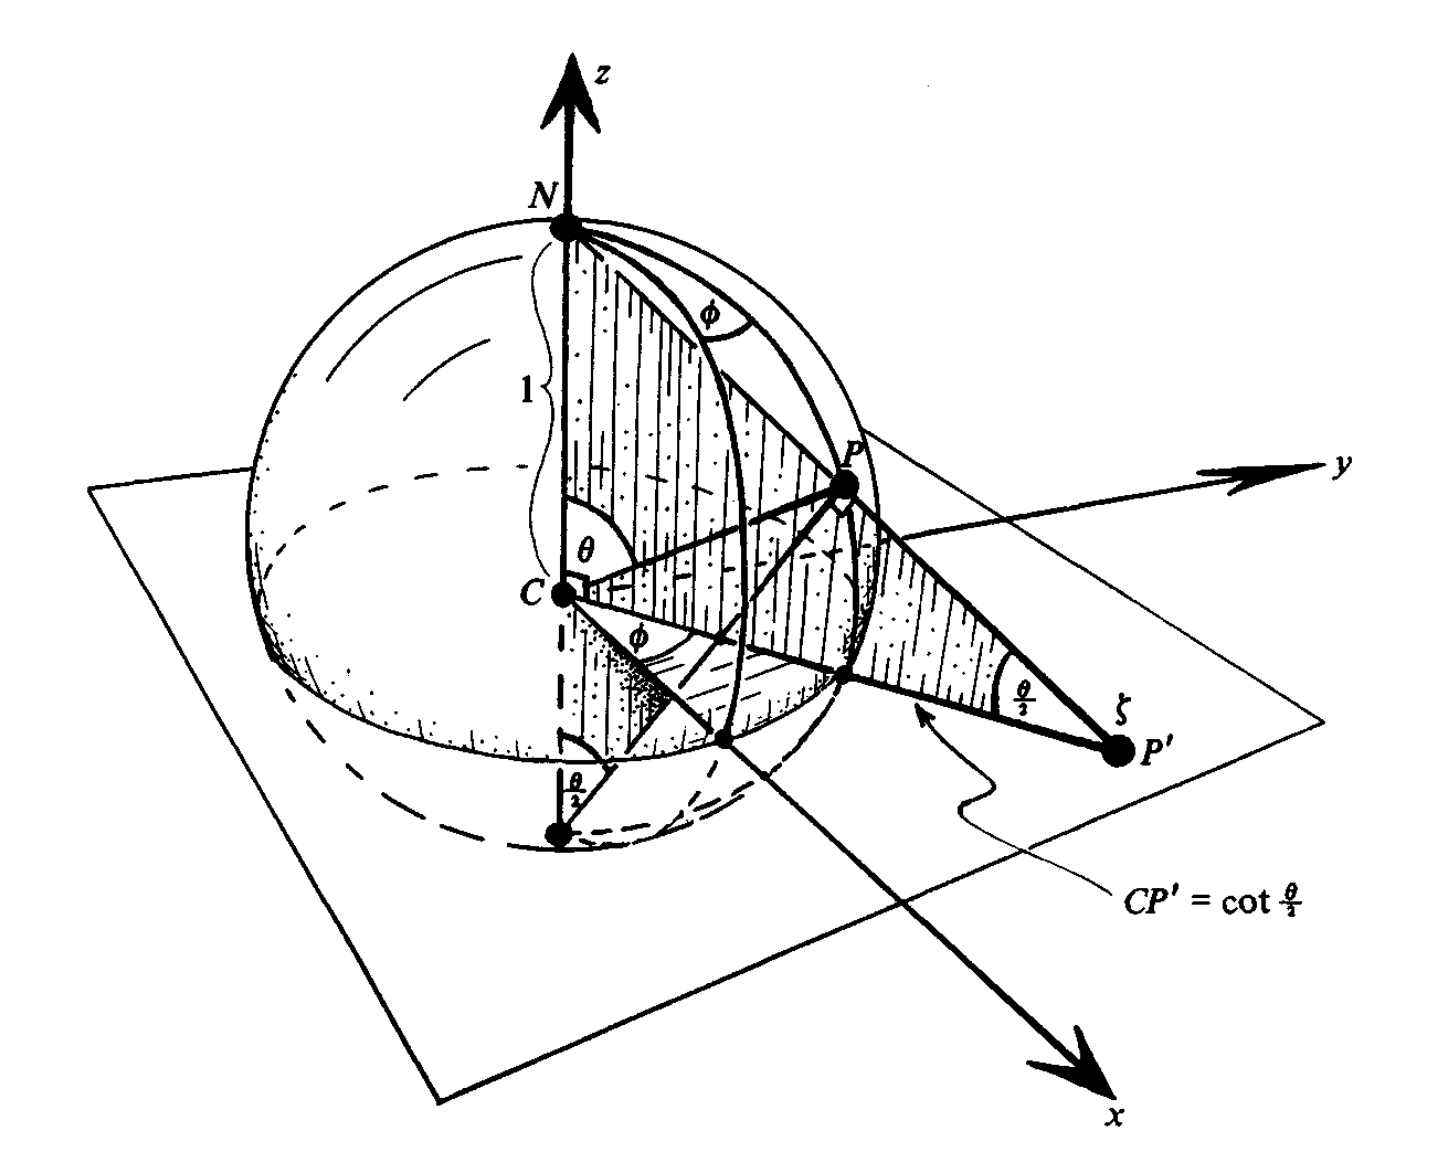
\includegraphics[width=10cm]{fig1-4.png}
    \caption{将球极角e与复立体坐标联系起来的方程=eit cot 8/2的几何形状。(角CP′n等于在南极处PN所补的角,因为两者都与角PNC互补。)}\label{fig:1-4}
\end{figure}
\begin{equation}
    x=\frac{\zeta+\bar{\zeta}}{\zeta\bar{\zeta}+1},y=\frac{\zeta-\bar{\zeta}}{\mathrm{i}(\zeta\bar{\zeta}+1)},z=\frac{\zeta\bar{\zeta}-1}{\zeta\bar{\zeta}+1}\label{eq:128}
\end{equation}

方程(\ref{eq:126})和(\ref{eq:128})给出了从$\zeta$所在的复平面到$(x, y, z)$-空间中球心为$(0,0,0)$的单位球上的标准的球极对应。我们把$\zeta=\infty$作为一个“点”添加到复平面上,并把这个点和球体的北极联系起来,这样就提供了一种一一的对应关系。用这种方法球面$S^+$给出了带有$\zeta=\infty$的$\zeta$复平面的标准实现:它就是$\zeta$的\textbf{黎曼球面}。

作为$S^+$的传统坐标化,我们还可以使用标准球坐标
\begin{equation}
    x= \sin \theta\cos \phi,y= \sin\theta\sin\phi, z=\cos\theta\label{eq:129}
\end{equation}
为了找到\(\zeta\)和$(\theta,\phi)$之间的关系,我们(\ref{eq:129})代入(\ref{eq:126})发现
\begin{equation}
    \zeta=e^{\mathrm{i}\phi} \cot \frac{\theta}{2}\label{eq:1210}
\end{equation}
这种关系也可以用一些三角知识直接得到,参考图\ref{fig:1-4}。
\begin{figure}
    \centering
    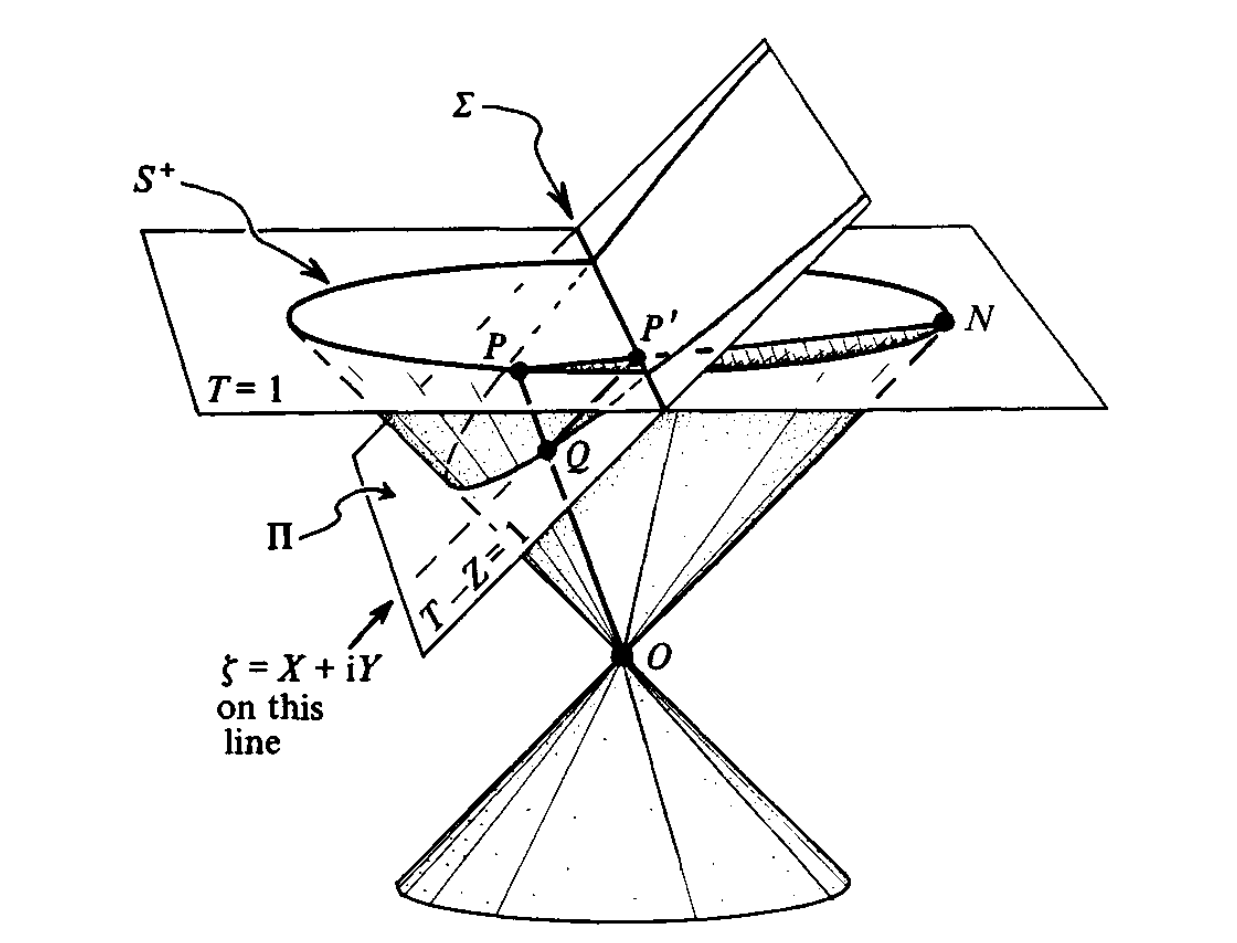
\includegraphics[width=10cm]{fig1-5.png}
    \caption{当通过ON的平面变化时,它提供了立体投影PHP'以及对应的P-Q和Q-P'。(I与圆锥的“抛物线”交点与平面(c的复平面)具有相同的固有欧几里得度规。)}\label{fig:1-5}
\end{figure}
公式(\ref{eq:126}),(\ref{eq:127}),(\ref{eq:128}),(\ref{eq:1210})适用于反天空映射
\[\text{未来光锥}\rightarrow S^+\rightarrow\Sigma\]
我们还对天空映射所对应的公式感兴趣,在$O$点的每一个类光方向代表一个典型的过去事件$-(1,x, y, z)$而不是一个未来事件$+ (1,x, y, z)$。如果我们需要在这两种情况下表示相同的类光直线,那么在$S^+$和$S^-$它必须对应于对跖点$\pm (x, y, z)$。所以我们可以通过对跖变换$(x, y, z)\mapsto-(x, y, z)$或是$(\theta,\phi )\mapsto(\pi-\theta,\pi+\theta )$从(\ref{eq:126})(\ref{eq:127})(\ref{eq:128})(\ref{eq:1210})获得相关的公式,特别地,方程(\ref{eq:1210})变成
\begin{equation}
    \zeta=-e^{\mathrm{i}\phi} \tan \frac{\theta}{2}\label{eq:1211}
\end{equation}
(注意,对跖点映射的效果是$\zeta\mapsto-1/\bar{\zeta} $)

上述在O点的未来[过去]类光方向集合与$\zeta$复平面之间的对应关系可以比通过球极投影更直接地得到。为了实现这种直接对应(见图\ref{fig:1-5}),我们把(T, X, Y, Z)空间与一个类光超平面$\Pi$相交,其方程为
\begin{equation}
    T-Z = 1
\end{equation}
而不是空间超平面$T = 1$。考虑一条通过O的零直线,在点$P= (1, x, y, z)$处与$S$相交。这条类光直线显然也包含$\Pi$平面上的点
\[Q=(\frac{1}{1-z},\frac{x}{1-z},\frac{y}{1-z},\frac{z}{1-z})\]
于是$Q$的“$x$”和“$y$”坐标是精确的
\[X'=\frac{1}{1-z}\text{和}\quad Y'=\frac{y}{1-z}\]
所以
\[\zeta=X'+\mathrm{i}Y'\]
如(\ref{eq:124})和(\ref{eq:126}),$\zeta$是由$\Pi$到$\Sigma$的简单正交投影得到的。在特例$\zeta=\infty (z=1)$的情况下,穿过O点的类光直线平行于$\Pi$,因此他们相交于无穷远。

我们参照图\ref{fig:1-5}来说明两个不同结构之间的几何关系。如前所述,设$N=(1,0,0,1)$是$s^+$的北极。设$OPQ$为考虑的类光直线,$P\in S^+$, $Q\in \Pi$。设$P'$为$Q$在平面$\Sigma(T= 1,Z=0)$上的正交投影。那么$QP'$的方向是$1:0:0:1$,与$ON$相同。因此$P',Q, O, N$是共面的。P在他们所在的平面上,因为它在$OQ$上。$P',P',N$也在超平面$T =1$上。因此它们共线\footnote{在四维下,一个平面(一个线性方程)和一个超平面(两个线性方程)的交是一条直线},由此得出$P'$是$P$(从$S^+$到$\Sigma$,以$N$为极点)的立体投影。因此,我们所需的等价性就这样用几何方法建立了。
\subsection*{洛伦兹变换和自旋变换}
为了避免$S^+$的北极点$(1,0,0,1)$也就是无穷远点$(\zeta=\infty)$方便的做法是不是由一个复数$\zeta$,而是由一对的(不同时为零的)复数$(\xi,\eta)$来标记$S^+$上的点,其中
\begin{equation}
    \zeta = \frac{\xi}{\eta}\label{eq:1213}
\end{equation}
这称为复射影(齐次)坐标,因此$(\xi,\eta)$和$(\lambda\xi,\lambda\eta)$表示$S^+$上的同一个点,其中$\lambda$是任意非零复数。在这种坐标下,无穷远点$\zeta=\infty $被赋予一个有限的标签,例如(1,0)。因此,我们现在把S+看作是一个复射影直线的实现。方程(\ref{eq:128})用复齐次坐标表示为
\begin{equation}
    x=\frac{\xi\bar{\eta}+\eta\bar{\xi}}{\xi\bar{\xi}+\eta\bar{\eta}},y=\frac{\xi\bar{\eta}-\eta\bar{\xi}}{\mathrm{i}(\xi\bar{\xi}+\eta\bar{\eta})},z=\frac{\xi\bar{\xi}-\eta\bar{\eta}}{\xi\bar{\xi}+\eta\bar{\eta}}\label{eq:1214}
\end{equation}
注意,$x$,$y,$和$z$关于$\xi,\eta$是齐次的,所以在$\xi,\eta$等比例缩放下是不变的。

回想一下,点$P(1, x, y, z)$在$S^+$上的作用就是表示$O$处的未来类光方向。如果愿意,我们可以选择直线$OP$上的任何其他点来表示相同的零方向。特别地,我们可以选择$OP$上的点$R$,其坐标$(T, X, Y, Z)$是由P的坐标乘以因子$(\xi\bar{\xi}+\eta\bar{\eta})/\sqrt{2}$得到的。这会去掉(\ref{eq:1214})中的分母。(为了以后方便,这里还包括了因子$1/\sqrt{2}$。)那么$\mathbf{K}:=\overrightarrow{OR}$有坐标
\begin{align}
    T=\frac{1}{\sqrt{2}}(\xi\bar{\xi}+\eta\bar{\eta}),\quad &X=\frac{1}{\sqrt{2}}(\xi\bar{\eta}+\eta\bar{\xi}),\nonumber\\
    Y=\frac{1}{\mathrm{i}\sqrt{2}}(\xi\bar{\eta}-\eta\bar{\xi}),\quad&Z=\frac{1}{\sqrt{2}}(\xi\bar{\xi}-\eta\bar{\eta}).\label{eq:1215}
\end{align}
不像 $P$点,$R$点并不依赖$(\xi,\eta)$的(实数)等比例缩放,即$(\xi,\eta)→(r\xi,r\eta),r\in R$,它还与相位“缩放”$(\xi,\eta)→(e^{\mathrm{i}\theta}\xi,e^{\mathrm{i}\theta}\eta),\theta\in R$无关。因此,尽管$OQ$的方向仅仅依赖于$\zeta$,但$\mathbf{R}$的位置并不仅仅是$\zeta$的函数。
现在从(\ref{eq:1215})不难看出,$\xi$和$\eta$的任何复线性变换都会造成$(T, X, Y, z)$的实线性变换(见下文(\ref{eq:1226}))。因为类光向量张成整个空间$\mathbb{V}$,类光向量的线性变换诱导出$\mathbb{V}$上在普通坐标$(T, X, Y, Z)$下的线性变换,由同一方程(即(\ref{eq:1226}))给出。这个变换下保持性质(\ref{eq:122})不变。这样我们就得到了一个洛伦兹变换,很可能还带有一个矢量大小的缩放。在任何情况下,对$O$点类光方向的影响将与洛伦兹变换的影响相同,因为缩放对方向没有影响。

那么,考虑一个$\xi$和$\eta$的复线性(非奇异)变换:
\begin{equation}
    \begin{split}
        \xi &\mapsto \tilde{\xi}=\alpha\xi +\beta\eta \\
        \eta &\mapsto \tilde{\eta}=\gamma\xi +\delta\eta
    \end{split}\label{eq:1216}
\end{equation}
这里,$\alpha, \beta, \gamma$和$\delta$是仅受$\alpha\delta-\beta\gamma\neq 0$(非奇点)条件约束的任意复数。变换(\ref{eq:1216})用$\zeta$表示为\footnote{这类双线性变换实际上是最一般的全局全纯(即复解析,也即保角和保定向)的黎曼球到自身的变换。}
\begin{equation}
    \zeta \mapsto \tilde{\zeta}=\frac{\alpha\zeta +\beta}{\gamma\zeta +\delta}\label{eq:1217}
\end{equation}
对于$\zeta$的变换,我们可以在不失一般性的情况下,通过施加“幺模”条件来规范化(\ref{eq:1216})
\begin{equation}
    \alpha\delta-\beta\gamma=1\label{eq:1218}
\end{equation}
根据(\ref{eq:1218}),变换(\ref{eq:1216})(或(\ref{eq:1217})),在通过方程(\ref{eq:1213})和(\ref{eq:1215})与闵可夫斯基类光向量相关的情况下,称为\textbf{自旋变换}。我们注意到
\begin{equation}
    \zeta = \frac{X+\mathrm{i}Y}{T-Z}=\frac{T+Z}{X-\mathrm{i}Y}\label{eq:1219}
\end{equation}
在同样的情况下,我们定义自旋矩阵$\mathbf{A}$为
\begin{equation}
    \mathbf{A}:=\begin{pmatrix}
        \alpha&\beta\\\gamma&\delta
    \end{pmatrix},\quad \det{\mathbf{A}}=1 \label{eq:1220}
\end{equation}
最后一个条件就是规范条件(\ref{eq:1218})。对于$\mathbf{A}$,(\ref{eq:1216})写成
\begin{equation}
    \begin{pmatrix}
        \tilde{\xi}\\\tilde{\eta}
    \end{pmatrix}=\mathbf{A}\begin{pmatrix}
        \xi\\\eta
    \end{pmatrix}\label{eq:1221}
\end{equation}
从(\ref{eq:1221})可以看出,两个连续自旋变换的组合同样是一个自旋变换:组合的自旋矩阵由因子的自旋矩阵的乘积给出。同时,任何自旋矩阵都有逆,
\begin{equation}
    \mathbf{A}^{-1}=\begin{pmatrix}
        \delta&-\gamma\\-\beta&\alpha
    \end{pmatrix}
\end{equation}
这也是一个自旋矩阵。因此,自旋变换形成一个群,称为$SL(2,\mathbb{C})$。

注意,自旋矩阵$\mathbf{A}$和-$\mathbf{A}$对$\zeta$产生相同的变换,即使它们定义不同的自旋变换。
反过来,假设$\mathbf{A}$和$\mathbf{B}$是自旋矩阵,它们分别定义了$\zeta$的相同变换,那么$\mathbf{B}^{-1}\mathbf{A}$是一个自旋矩阵,它定义了$\zeta$上的恒等变换。由(\ref{eq:1217})可知$\beta=\gamma=0, \alpha=\delta$。规范条件(\ref{eq:1218})意味着$\alpha=\beta= \pm 1$。因此$\mathbf{B}^{-1}\mathbf{A}=±\mathbf{I}$(单位矩阵),其中$\mathbf{A}=\pm \mathbf{B}$。自旋变换因此被唯一地定义为它对$\zeta$的黎曼球面的影响。

让我们考察自旋变换(\ref{eq:1221})对坐标$(T, X, Y, Z)$的影响。我们观察到(\ref{eq:1215})可以被反解并重新表示为:
\begin{equation}
    \frac{1}{\sqrt{2}}
    \begin{pmatrix}
        T+Z&X+\mathrm{i}Y\\
        X-\mathrm{i}Y&T-Z
    \end{pmatrix}=
    \begin{pmatrix}
        \xi\bar{\xi}&\xi\bar{\eta}\\
        \eta\bar{\xi}&\eta\bar{\eta}
    \end{pmatrix}=
    \begin{pmatrix}
        \xi\\
        \eta
    \end{pmatrix}\begin{pmatrix}
        \bar{\xi}&\bar{\eta}
    \end{pmatrix}
\end{equation}
由此,我们可以看到自旋变换(\ref{eq:1121})导致:
\begin{equation}
    \begin{pmatrix}
        T+Z&X+\mathrm{i}Y\\
        X-\mathrm{i}Y&T-Z
    \end{pmatrix}\mapsto\begin{pmatrix}
        \tilde{T}+\tilde{Z}&\tilde{X}+\mathrm{i}\tilde{Y}\\
        \tilde{X}-\mathrm{i}\tilde{Y}&\tilde{T}-\tilde{Z}
    \end{pmatrix}=\mathbf{A}\begin{pmatrix}
        T+Z&X+\mathrm{i}Y\\
        X-\mathrm{i}Y&T-Z
    \end{pmatrix}\mathbf{A}^\dagger \label{eq:1224}
\end{equation}

其中$A^\dagger$表示$A$的共轭转置。如前所述,这是$(T, X, Y, Z)$的一个线性变换,它是实数(因为在(\ref{eq:1224})中保留了厄米性),并且它也满足$T^2-X^2-Y^2-Z^2=0$
同样,如果
\begin{equation}
    \mathbf{U} = T\mathbf{t} + X\mathbf{x} + Y\mathbf{y} + Z\mathbf{z}\label{eq:1225}
\end{equation}
是任何世界向量(不必要是类光的),那么自旋矩阵$\mathbf{A}$仍然是根据(\ref{eq:1224})定义的$\mathbf{U}$的变换。我们注意到这个变换不仅是实线性的,而且它还使$T^2-X^2-Y^2-Z^2$保持形式不变。这个形式就是(\ref{eq:1224})中左边矩阵的行列式,而右边的行列式就是这个形式乘以$\det \mathbf{A} \det \mathbf{A^\dagger}=1$ (参见(\ref{eq:1220}))。因此(\ref{eq:1224})定义了一个洛伦兹变换。作为$(T,X,Y,Z)$上的变换,其显式形式为
\begin{gather}
        \begin{pmatrix}
            T\\X\\Y\\Z
        \end{pmatrix}\mapsto
        \begin{pmatrix}
            \tilde{T}\\\tilde{X}\\\tilde{Y}\\\tilde{Z}
        \end{pmatrix}=\frac{1}{2}\mathbf{B}
        \begin{pmatrix}
            T\\X\\Y\\Z
        \end{pmatrix},\nonumber\\
        \mathbf{B}=
        \small{\small{\begin{pmatrix} 
            \alpha  \bar{\alpha }+\beta  \bar{\beta }+\gamma  \bar{\gamma }+\delta  \bar{\delta }& \beta  \bar{\alpha}+\alpha  \bar{\beta }+\delta  \bar{\gamma }+\gamma  \bar{\delta }& -\mathrm{i} \beta  \bar{\alpha }+\mathrm{i} \alpha  \bar{\beta }-\mathrm{i}\delta  \bar{\gamma }+\mathrm{i} \gamma  \bar{\delta }& \alpha  \bar{\alpha }-\beta  \bar{\beta }+\gamma  \bar{\gamma }-\delta \bar{\delta }\\
            \gamma  \bar{\alpha }+\alpha  \bar{\gamma }+\delta  \bar{\beta }+\beta  \bar{\delta }& \delta\bar{\alpha }+\alpha  \bar{\delta }+\gamma  \bar{\beta }+\beta  \bar{\gamma }& -\mathrm{i} \delta  \bar{\alpha }+\mathrm{i} \alpha \bar{\delta }+\mathrm{i} \gamma  \bar{\beta }-\mathrm{i} \beta  \bar{\gamma }& \gamma  \bar{\alpha }+\alpha  \bar{\gamma }-\delta \bar{\beta }-\beta  \bar{\delta }\\ 
            \mathrm{i} \gamma  \bar{\alpha }-\mathrm{i} \alpha  \bar{\gamma }+\mathrm{i} \delta  \bar{\beta }-\mathrm{i} \beta \bar{\delta }& \mathrm{i} \delta  \bar{\alpha }-\mathrm{i} \alpha  \bar{\delta }+\mathrm{i} \gamma  \bar{\beta }-\mathrm{i} \beta  \bar{\gamma }&\delta  \bar{\alpha }+\alpha  \bar{\delta }-\gamma  \bar{\beta }-\beta  \bar{\gamma }& \mathrm{i} \gamma  \bar{\alpha }-\mathrm{i}\alpha  \bar{\gamma }-\mathrm{i} \delta  \bar{\beta }+\mathrm{i} \beta  \bar{\delta }\\ 
            \alpha  \bar{\alpha }+\beta  \bar{\beta }-\gamma \bar{\gamma }-\delta  \bar{\delta }& \beta  \bar{\alpha }+\alpha  \bar{\beta }-\delta  \bar{\gamma }-\gamma  \bar{\delta}& -\mathrm{i} \beta  \bar{\alpha }+\mathrm{i} \alpha  \bar{\beta }+ \delta  \bar{\gamma }-\mathrm{i} \gamma  \bar{\delta }& \alpha \bar{\alpha }-\beta  \bar{\beta }-\gamma  \bar{\gamma }+\delta  \bar{\delta }
        \end{pmatrix}}}\label{eq:1226}
\end{gather}
事实上,这一定是一个受限洛伦兹变换。因为:(i)一个带有恒等元的连续的洛伦兹变换一定是受限的。因为不存在连续的洛伦兹运动能够将正时间轴从未来光锥变到过去光锥里,或是实现空间反射:(ii)变换(\ref{eq:1224})显然是一个带有恒等元的连续变换;(iii)$\mathbf{A}$像每个自旋矩阵一样,可以连续地变换到单位矩阵。考虑矩阵$\mathbf{B}:=\lambda \mathbf{I}+(1- \lambda)\mathbf{A}$由于它对$\lambda$的至多两个值是奇异的,我们可以在复$\lambda$平面中找到一条从0到1的路径来避开这些奇异的值。考虑$(\det \mathbf{B})^{-\frac12}\mathbf{B}$定义了从$\mathbf{A}$到$\mathbf{I}$或$-\mathbf{I}$的连续自旋变换。(要想变到$-\mathbf{I}$,那这个路径就要使得$(\det \mathbf{B})$从$-1$变到$1$,这是容易实现的,例如,若$A=-I$。自旋变换$\text{diag}(e^{\mathrm{i}\theta},e^{-\mathrm{i}\theta}),0\leqslant\theta\leqslant\pi $可以让$-I$到$I$是连续的),这样(iii)就建立起来了

我们将给出一个建设性的证明,相反地,任何受限的洛伦兹变换都可以用(\ref{eq:1224})的形式用一个自旋矩阵表示。那么我们就得到了以下的基本结果:
\begin{proposition}
每个自旋变换对应(通过(\ref{eq:1224}))一个唯一的受限洛伦兹变换;反过来说,每个受限洛伦兹变换同时与两个这样的自旋变换相对应,它们的符号相反。\label{pro:1227}
\end{proposition}

实际上,这个结果的逆命题部分是李群一般性质的一个简单推论。洛伦兹群的子群的形式出现(\ref{eq:1224})必须有完整的维数6,这是因为自旋矩阵形成6实维(即3复维)系统,又因为自旋矩阵定义的洛伦兹变换只有一个离散的参数(这个参数只取两个值)。这个全维子群必须包含洛伦兹群中恒等元的全部连通分量。

然而,给出命题\ref{pro:1227}逆命题部分的另一种证明是有意义的,方法是简单明确地构造那些自旋矩阵,这些自旋矩阵对应于某些足以产生整个群的基本洛伦兹变换。这些基本的转换是空间旋转和“boost”(即纯粹的速度变换)
\begin{equation}
    \tilde{T} = \frac{T+vZ}{\sqrt{1-v^2}}, \tilde{X} = X,  \tilde{Y}=Y, \tilde{Z} = \frac{Z+vT}{\sqrt{1-v^2}}\label{eq:1228}
\end{equation}
其中$v$是速度参数。任何受限的(主动)洛伦兹变换都可以由适当的空间旋转,然后$Z$方向boost,最后再来一次空间旋转组合而成,因为这样的变换对Minkovski基的作用是特征的。让第一个旋转把$z$带入进初始和最终$\mathbf{t}$方向所确定的时空平面。boost(1.2.28)将$\mathbf{t}$入最终方向,第二个旋转适当地还原$\mathbf{x},\mathbf{y}$和$\mathbf{z}$。因此,我们只需要证明空间旋转和$z-boost$可以通过自旋变换获得。我们首先考虑旋转问题,事实上,有下面的结果:
\begin{proposition}
    每个酉自旋变换对应着$S^+$的唯一固有旋转;相反地,$S^+$的每一个固有旋转恰好对应于两个符号相反的酉自旋变,。(酉自旋变换是由酉自旋矩阵给出的:$A^{-1}=A^\dagger$)\label{pro:1229}
\end{proposition}

首先,让我们进一步确定一下这些变换的几何意义。洛伦兹变换在这里是主动的。球面$S^+$和$S^-$是坐标系的一部分,不参与变换:当每一个未来[过去]的类光方向被移位时,它在$S^-$上的表示也会移位。
例如,$\mathbf{(x, y, z)}$的旋转使$\mathbf{t}$不变,对应于$S^+[S^-]$上的旋转的像,我们可以松散地称之为$S^+[S^-]$“的”旋转。平面$\Sigma$也是坐标结构的一部分,当类光直线的像在它上面移动时,它仍然是固定的。同样,我们也可以笼统地说这是$\Sigma$“的”的运动(当然相比起各种坐标超平面,$S^+,S^-,\Sigma$看起来并没有那么地“不变”:在洛伦兹变换下,在$S^+,S^-,\Sigma$上终止的向量通常不会变。)
重要的是要记住,虽然我们这里只有$\mathbb{V}$的类光方向的表示,但它们的变换却唯一地决定了$\mathbb{V}$中所有向量的变换。

现在从(\ref{eq:1224})可知,$T$在酉自旋变换下是不变的,因为迹($=2T$)在幺正变换下总是不变的。(等价地,我们可以从表达式$\xi\bar{\xi}+\eta\bar{\eta}$的不变性看出这一点,它是$(\xi,\eta)$的厄米范数。)T不变的受限洛伦兹变换是$S+$的恰当旋转(因为它们保持$X^2 + Y^2 + Z^2$不变)。
为了明确地证明相反的情况,我们首先注意到$S^+$的任何适当旋转$(x,y,z)\mapsto(x',y',x')$都可能是围绕$y$轴和$z$轴连续旋转的复合。对于空间基$(\mathbf{x', y',z'})$是由$\mathbf{z'}$相对于$(\mathbf{(x,y,z)})$的极坐标$\theta,\phi$和$\mathbf{x', z'}$平面对$\mathbf{z, z'}$的角度$\psi$决定的。(这三个角度本质上就是著名的力学欧拉角:参见Goldstein 1980和Arnold 1978)。因此,绕$\mathbf{z}$旋转$\psi$,然后绕原来的$\mathbf{y}$旋转$\theta$,最后绕原来的$\mathbf{z}$旋转$\phi$,就可以得到所需的变换。我们将说明如何用幺正自旋变换来表示这些基本的旋转。由此可以得出,$S^+$的任何适当旋转都可以这样表示,因为酉矩阵的乘积还是酉的。

$S^+$绕$z$轴旋转一个角度,显然来自于复平面绕原点旋转一个角度。
由下式给出
\begin{equation}
    \tilde{\zeta}=e^{\mathrm{i}\psi}\zeta\label{eq:1230}
\end{equation}
即通过自旋变换
\begin{equation}
    \begin{pmatrix}
        \tilde{\xi}\\\tilde{\eta}
    \end{pmatrix}=\pm \begin{pmatrix}
        e^{\mathrm{i}\psi/2}&0\\0&e^{-\mathrm{i}\psi/2}
    \end{pmatrix}\begin{pmatrix}
        \xi\\\eta
    \end{pmatrix}\label{eq:1231}
\end{equation}
接下来,我们断言$S^+$绕$y$轴旋转$\theta$角是由以下酉自旋变换表示的:
\begin{equation}
    \begin{pmatrix}
        \tilde{\xi}\\\tilde{\eta}
    \end{pmatrix}=\pm \begin{pmatrix}
        \cos\theta/2&-\sin\theta/2\\\sin\theta/2&\cos\theta/2
    \end{pmatrix}\begin{pmatrix}
        \xi\\\eta
    \end{pmatrix}\label{eq:1232}
\end{equation}
由于(\ref{eq:1232})是酉的,它当然代表了某种旋转。此外,因为除$\xi\bar{\xi}+\eta\bar{\eta}$外$\xi\bar{\eta}-\eta\bar{\xi}$也是不变的,由(\ref{eq:1214})可知$S^+$上点的$y$坐标在(\ref{eq:1232})下是不变的。因此旋转是绕$y$轴的。最后,变换(\ref{eq:1232})将点$(1,0,0,1)$变为$(1,\sin\theta,0, \cos \theta)$,因此旋转角度确实是$\theta$。类似地,可以验证,酉自旋变换
\begin{equation}
    \begin{pmatrix}
        \tilde{\xi}\\\tilde{\eta}
    \end{pmatrix}=\pm \begin{pmatrix}
        \cos\chi /2&\mathrm{i}\sin\chi /2\\\mathrm{i}\sin\chi /2&\cos\chi /2
    \end{pmatrix}\begin{pmatrix}
        \xi\\\eta
    \end{pmatrix}\label{eq:1233}
\end{equation}
对应于绕x轴旋转一个角度$\chi$。

命题\ref{pro:1229}现在成立。作为参考,我们展示了通过欧拉角$\theta,\phi,\chi$对应于(一般)旋转的合成自旋矩阵
\begin{equation}
    \pm \begin{pmatrix}
        \cos\frac{\theta}{2} e^{\mathrm{i}(\phi+\psi)/2}&-\sin\frac{\theta}{2} e^{\mathrm{i}(\phi-\psi)/2}\\\sin\frac{\theta}{2} e^{-\mathrm{i}(\phi-\psi)/2}&\cos\frac{\theta}{2} e^{-\mathrm{i}(\phi+\psi)/2}
    \end{pmatrix}
\end{equation}
它的元素实际上是力学上的Cayley-Klein旋转参数。参见Goldstein(1980)。

现在只需要证明每个z-boost(\ref{eq:1228})都可以从自旋变换中得到,我们就完成了命题\ref{pro:1227}的证明。要做到这一点,我们重写(\ref{eq:1228})
\begin{equation}
    \tilde{T}+\tilde{Z} = w{(T+Z)},\tilde{T}-\tilde{Z} = w^{-1}({T+Z}), \tilde{X} = X,  \tilde{Y}=Y\label{eq:1235}
\end{equation}
其中
\begin{equation}
    w=\sqrt{\frac{1+v}{1-v}}
\end{equation}
(这里$w$是相对论多普勒因子,$\ln w = \tanh^{-1} v$是对应于v的“快度”)通过(\ref{eq:1224}),我们看到(\ref{eq:1235})是由如下自旋变换实现的
\begin{equation}
    \begin{pmatrix}
        \tilde{\xi}\\\tilde{\eta}
    \end{pmatrix}=\pm \begin{pmatrix}
        \sqrt{w}&0\\0&\frac{1}{\sqrt{w}}
    \end{pmatrix}\begin{pmatrix}
        \xi\\\eta
    \end{pmatrix}\label{eq:1237}
\end{equation}
或者,对于$\zeta$的复平面,可以简单写成。
\begin{equation}
    \tilde{\zeta}=w\zeta \label{eq:1238}
\end{equation}
命题\ref{pro:1227}由此成立。
我们最后指出,任何纯boost(两个与$\mathbf{t}$垂直的超平面保持不变,例如上面的$X =0, Y =0$)对应于一个正的或负的厄米自旋矩阵,反之亦然。对z-boost(\ref{eq:1237})就是这种形式,为了获得其他方向的boost,我们只需要将这个方向旋转到$z$方向,应用z-boost,然后旋转回来。这对应于自旋矩阵$\mathbf{A}^{-1}\mathbf{B}\mathbf{A}$,其中$\mathbf{A}$是所需的旋转,$\mathbf{B}$是z-boost;根据初等矩阵理论,$\mathbf{A}^\dagger \mathbf{B}\mathbf{A}$仍然是正负定的厄米矩阵。相反地,任何正负定厄米矩阵$\tilde{\mathbf{B}}$都可以由一个酉矩阵$\mathbf{A}$对角化:$\mathbf{A}\tilde{\mathbf{B}}\mathbf{A}^{-1}= \text{diag}(\alpha,\delta)$,其形式必须是$\pm \text{diag}(w^{\frac12},w^{-\frac12})=±\mathbf{B}$,因为厄米性、定性和单位行列式得以保留。因此$\tilde{\mathbf{B}}$的形式为$\pm \mathbf{A}^{-1}\mathbf{B}\mathbf{A}$,我们的结果随即成立。

从前面的工作中很容易看出,任何受限的洛伦兹变换$L$都是由一个boost推力和一个适当的空间旋转组成的唯一组合,反之亦然。因为我们只需要确定包含初始$\mathbf{t}$和最终$\mathbf{t}$的平面中与$\mathbf{t}$正交的空间方向$\mathbf{w}$,应用一个“$\mathbf{w}$-boost”将$t$送入其最终位置,然后应用一个空间旋转来适当地重新定位$x, y,z$\footnote{由此可知,受限洛伦兹群的拓扑是旋转群与R的拓扑积。}。显然,如果我们反向执行这些变换,我们就得到了$L^{-1}$的分解。再来看看之前的研究。读者将在这个结果中认识到一个数学定理的例子,根据这个定理,任何非奇异复矩阵都可以唯一地写成一个酉矩阵和一个正定厄米矩阵的乘积,反之亦然。
\subsection*{和四元数的关系}
虽然酉自旋矩阵和单位四元数实际上是一回事,但一般来说,自旋矩阵和四元数之间并没有如此密切的关系。这背后的原因是四元数与正定号差的二次形式相关联(cf。(1.2.45))而自旋矩阵和洛伦兹变换与洛伦兹号差($+,-,-,-)$有关。当然,我们可以通过引入带有适当复系数的“四元数”来避免这种困难。这样的对象与实四元数不具有构成除法代数的基本性质。然而,仅仅使用四元数记数法(特别是(1.2.47))就可以为一般自旋矩阵的某些操作带来相当大的好处(参见,例如,Ehlers, Rindler和Robinson 1966)。
\section{洛伦兹变换的一些性质}\label{sec.1.3}
由于受限制的洛伦兹群和自旋变换群之间的对应关系,有可能给出许多旋转和洛伦兹变换的标准性质的简单推导,这就是我们现在要做的。

很容易看出,当自旋变换(\ref{eq:1216})为酉的时,(\ref{eq:1217})变为
\begin{equation}
    \zeta \mapsto \tilde{\zeta}=\frac{\alpha\zeta -\bar{\delta}}{\gamma\zeta +\bar{\alpha}}\label{eq:131}
\end{equation}
不动点($\tilde{\zeta}=\zeta$)则由下式给出
\begin{equation*}
    \gamma\zeta^2+(\bar{\alpha}-\alpha)\zeta+\bar{\gamma}
\end{equation*}
显然,如果$\zeta $是这个二次方程的一个根,那么$-1/\bar{\zeta}$就是另一个根。
因此,不动点的形式为$\zeta $, $-1/\bar{\zeta}$,对应于球$S^+$上的对跖点(参见(\ref{eq:1211})之后)。这又证明了球面的每一次旋转都等价于绕单一轴旋转

球面$S^+$上的圆被定义为$S^+$与$T= 1$时欧氏三维空间中的某个平面的交点,该平面由一个实的线性方程$lX+mY+ nZ=p(p^2 < l^2+ m^2 + n^2)$给出。代入(\ref{eq:128}),我们得到$(\text{给定}p\neq n)$如下形式的一个方程,$\zeta\bar{\zeta}-\kappa\bar{\zeta}-\zeta\bar{\kappa}+ \kappa\bar{\kappa}=r^2 (r>0, \kappa\text{是复数})$,即$|\zeta-\kappa|=r$。这是复平面上圆心为$\kappa $,半径为$r$的圆的方程。当$p=n$时(也就是当原来的圆经过$S^+$上的北极时),我们得到
复平面上的一条直线。因此,我们已经建立了一个众所周知的事实,即球面上的圆映射为平面上的圆或直线,反之亦然,因为上面的论述是可逆的

在前一节中,我们证明了每个自旋变换都可以由诱导$S^+$旋转或复平面简单扩展的变换组合而成。第一种在$S^+$上明显保留圆,第二种在平面复上明显保留圆或直线。因此,从上面的讨论可以得出,每个自旋变换都诱导了$S^+$上的一个变换,它把圆变成圆。(这实际上是黎曼球的双线性变换(\ref{eq:1217})的一个熟悉的性质,并不是很难直接建立。)

任何保圆变换都必须是共性(保角)的。这基本上是因为无限小的圆必须转换成无限小的圆,而不是椭圆。另外,我们也可以通过观察球面上的线长$\mathrm{d}\sigma^2 $与阿根平面上的$\mathrm{d}\zeta \mathrm{d}\bar{\zeta}$之间的关系来直接验证球极投影的保角性质
\begin{equation}
    \mathrm{d}\sigma^2 =\mathrm{d}x^2+\mathrm{d}y^2+\mathrm{d}z^2=\frac{4\mathrm{d}\zeta\mathrm{d}\bar{\zeta}}{(\zeta\bar{\zeta}+1)^2}
\end{equation}
如(\ref{eq:128})所示。双线性变换的保角性质可以从它是全纯的(即复解析的)\footnote{相反地,黎曼球的每一个局部固有(即保持方向)保角变换都来自于的全纯映射。(对于保形意味着$d,= ad$,对于复数a,即(dx +idi)=aldx + idv),由其推导出Cauchy-Riemann方程0x/ox = Re(a)-oj/ay,-otlay=Im(a)=0j/ox,因此holomorphicity。)由于黎曼球到自身的唯一全局全纯映射是双线性变换,因此,S*(通过St理解)到自身的唯一真正的全局保形映射是由自旋变换诱导的。因此,正的真保角自变换群是受限洛伦兹群。+的结构是有意义的,因此正是它的aOrmai构造与取向。
保形结构
事实上,任何2曲面
球面S和(正defínite)共形结构的拓扑与度规球面(说S+)共形相同。因此,T的真保角自变换也与限制洛伦兹群形成同构群。这个结果在第九章中对我们很重要
(ef。(9.6.31)}这一事实推导出来;$\tilde{\zeta}=f(\zeta)$可得$\mathrm{d}\tilde{\zeta}=f'(\zeta)\mathrm{d}\zeta$。由此可见,洛伦兹变换在$S^+$的每个点的邻域的作用是各向同性扩张和旋转

上述保角和保圆的性质的一个推论就是
我们熟悉却又不是那么熟悉的一个狭义相对论效应,有时被称为“洛伦兹收缩的不可见性”。让我们设想一个观察者在$O$。如前所述,他的视野(或天体)可能是,
为方便用$S^-$表示。进入他眼睛的每一束光线都用一条通过$O$的类光直线表示,因此用他的天球$S^-$(天空映射)的一个点表示。现在$S^-$和$S^+$仅仅通过对跖映射联系起来。因此,$\mathbb{V}$上的任何洛伦兹变换都可导出天球在自身上的共形保圆映射。根据保形性质,一个物体在一个观察者处与一个小角度相对时,将在视觉上呈现与其他观察者暂时重合的相似形状,不管他相对于第一个观察者的速度是多少(Terrell 1959)
一般来说,对于两个这样的观察者,只有表观角度大小和方向是不同的。 此外,根据保圆的性质,如果一个惯性观察者感知到任意尺寸的物体有一个圆形轮廓,那么所有与第一个惯性观察者暂时重合的惯性观察者都将感知到圆形轮廓(或在特殊情况下,如果我们认为天球上的一个大圆看起来是“直的”,那么它就是“直线轮廓”)。因此,特别地,在洛伦兹收缩的情况下,均匀运动的球体向所有观察者呈现圆形轮廓(彭罗斯1959)。

如果我们指定任意三个不同的点作为球面上任意其他三个不同点的像,黎曼球的双线性变换就完全确定了。这个众所周知的事实是(\ref{eq:1217})的简单结果。(三个复比$\alpha:\beta:\gamma:\delta$定义了这个变换,它们由三个复方程确定。)因此,如果我们指定三个不同类光方向的(不同)映射,则每个受限洛伦兹变换都是完全确定的。(因此,通过对速度和方向的适当调整,观测者可以使任意三颗给定的恒星在他的天球上占据三个特定的位置。)

同样,每个双线性变换(\ref{eq:1217})-不仅仅是特殊情况(\ref{eq:131})-(除了恒等变换)只在黎曼球上有两个(可能重合的)不动点,这很容易看到,如果我们在(\ref{eq:1217})中设$\bar{\zeta}=\zeta$并解得的二次方程。因此,每个(非平凡的)洛伦兹变换只留下两个(可能重合的)类光方向不变\footnote{
事实上,根据一个拓扑定理,球面在其自身上的每一个连续保持方向的映射必须至少有一个不动点,正确地计算,确切地说是两个不动点,因为球面的欧拉特征是2。可以对比\S 8.7中关于'fingerprints'的讨论。}

\subsection*{用$S^+$表示的洛伦兹变换}
让我们根据这个事实来研究洛伦兹变换的结构。首先考虑两个固定的类光方向不同的情况。
通过选择参考的闵可夫斯基基,我们可以得到这种洛伦兹变换的标准形式,使$\mathbf{t}$和$\mathbf{z}$位于由这些类光方向张成的2-平面上。后者必须有分量$(1,0,0,\pm 1)$,其中不动点位于$S^+ (\zeta=\infty, 0)$的南极和北极。使两个极点不变的最一般的双线性变换(\ref{eq:1217})有以下形式
\begin{equation}
    \tilde{\zeta}=we^{\mathrm{i}\psi }\zeta
\end{equation}
其中$w$和$\psi$为实数。这是由(顺序无所谓)绕z轴旋转一个角度$\psi$,与沿z轴的快度为$\phi=\ln w$的boost组成(参见图。\ref{fig:1-6}, \ref{fig:1-7}, \ref{fig:1-8})。就闵可夫斯基坐标\ref{eq:1215}而言,我们有
\begin{align}
    \tilde{X}=X \cos\psi-Y\sin\psi,&\tilde{Y}=X \sin\psi+Y\cos\psi,\nonumber\\
    \tilde{Z}=Z \cosh\phi+T\sinh\phi,&\tilde{T}=Z \sinh\phi+T\cosh\phi.
\end{align}
这就是Synge称作的“4-螺旋”(Synge, 1953, p. 86)

我们已经看到,$z$方向上的纯boost对应于复平面的膨胀$\tilde{\zeta}=w\zeta$。用天空映射($S^-$),并用球坐标作为天球(参见(\ref{eq:1211}),就有了入射光线的像差公式的有用形式:
\begin{align}
    \tan{\frac{\tilde{\theta}}{2}}&=w\tan{\frac{\theta}{2}}\nonumber\\
    w&=(\frac{1-V}{1+V})^{1/2}\
\end{align}
这里$V=-v$是测量角度$\tilde{\theta}$的观测者相对于测量角度为$\theta$的观测者在$\theta=0$方向上的速度。(由于我们的变换是主动的,我们必须认为宇宙的其余部分都获得了z方向上的速度$- V = v$。)我们看到,当一个观察者以很高的速度向恒星$P$行进时,他会察觉到其他恒星越来越多地聚集在$P$周围,他的速度也随之增加

接下来我们研究两个固定的类光方向重合的洛伦兹变换。这叫做类光旋转。在不失一般性的情况下,我们可以选择固定的类光方向来对应$S^+$的北极。因此=o是双线性变换(1.2.17)的唯一不动点,因此
了= 5 + p
(1.3.6)
其中B是某个复数。这只是阿甘平面上的翻译。(<=00为不动点的Argand平面的双线性变换必须为(=at +B,但如果A +1,它也有一个有限不动点)给出(1.3.6)的自旋变换为
) = t) (6) (
(1.3.7)
在不失一般性的前提下,我们可以取a为实数的B=ia。然后用闵可夫斯基坐标表示
x = x, r = Y + 2)
2 = Z + aY + (T-Z), T = T + aY +助教(2)。
(1.3.8)
请注意,零向量z + r本身是不变的,而不仅仅是它的方向。
1.3洛伦兹变换的性质
7
\section{零标和自旋矢量}\label{sec:1.4}
\section{旋量对象和自旋结构}
\section{旋量算符的几何}
\chapter{抽象指标和旋量代数}
\section{抽象指标方法的动机}
\section{张量代数的抽象指标形式}
\section{基}
\section{流形上G的全部自反性}
\section{旋量代数}
\chapter{旋量和世界张量}
\section{世界张量作为旋量}
\section{零标和复类光矢量}
\section{对称算符}
\section{旋量算符的张量表示}
\section{在同一观点下张量和旋量的简单主张}
\section{洛伦兹变换}
\chapter{微分和曲率}
\section{流形}
\section{协变导数}
\section{联络依赖的导数}
\section{旋量的微分}
\section{旋量分量的微分}
\section{曲率旋量}
\section{Einstein-Cartan-Sciama-Kibble理论的旋量表达}
\section{Weyl张量和Bel-Robinson张量}
\section{对易子的旋量形式}
\section{Bianchi恒等式的旋量形式}
\section{曲率旋量和自旋系数}
\section{紧凑的自旋系数形式}
\section{Cartan方法}
\section{在2-表面上的应用}
\section{自旋球谐函数}
\chapter{时空中的场}
\section{电磁场和它的导数算符}
\section{Einstein-Maxwell方程组的旋量形式}
\section{Rainich条件}
\section{矢量丛}
\section{杨-Mills场}
\section{共形缩放}
\section{一致性条件}
\section{各类场量的共形不变性}
\section{场的精确集}
\section{光锥上的初始数据}
\section{显式场积分}
\section*{附录:图形符号}
\end{document}